\documentclass[a4,11pt]{article}
\usepackage{geometry}
\geometry{a4paper, top=40mm, left=30mm, right=30mm, bottom=35mm}
\setlength\parindent{0pt}
\usepackage[german]{babel}
\usepackage[utf8]{inputenc}


\usepackage{multicol} % Spalten
\usepackage{color} % Farben
\usepackage[hyphens]{url} % Internetadresse (mit automatischer Trennung)
\usepackage{enumitem} % Aufzählungen


% Literaturverzeichnis
\usepackage{csquotes}
\usepackage{biblatex}
\addbibresource{../Allgemeines/Literatur.bib}


% Mathesymbole
\usepackage{amsmath, amsthm, amssymb}
\usepackage{bm} % fette Schrift in Matheumgebung
%\usepackage{physics} % Derivate richtig schreiben
%\usepackage[version=4]{mhchem} % Chemische Elemente
\usepackage[
	locale=DE,
	separate-uncertainty=true, % Fehler mit ±
	per-mode=symbol-or-fraction, % m/s im Text, sonst \frac
	% alternativ:
	% 	per-mode=reciprocal,
	% 	m s^{-1}
	output-decimal-marker=., % . statt , für Dezimalzahlen
	alsoload=synchem, % für \torr und andere chemische sachen
	]{siunitx} % si-Einheiten
	
% Chemiesymbole
\usepackage[version=3]{mhchem}

%Einfach Ableitungen etc.
\usepackage{physics}


% Bilder
\usepackage{caption}
\usepackage{graphicx, wrapfig}
\usepackage{subcaption} % Bilder in Gruppe einzeln benennen
\usepackage{tikz}
\usetikzlibrary{matrix} % zeigt Koordinatensystem an
\usepackage[european]{circuitikz} % Schaltkreise
\usetikzlibrary{arrows}
\newcommand{\mymeter}[2] % Option um Schaltsymbole zu drehen
{  % #1 = name , #2 = rotation angle
	\begin{scope}[transform shape,rotate=#2]
		\draw[thick] (#1)node(){$\mathbf V$} circle (11pt);
		\draw[rotate=45,-latex] (#1)  +(-17pt,0) --+(17pt,0);
	\end{scope}
}

\usepackage[
labelfont=bf,        % Tabelle x: Abbildung y: ist jetzt fett
font=small,          % Schrift etwas kleiner als Dokument
width=0.9\textwidth, % maximale Breite einer Caption schmaler
]{caption}
\sisetup{table-format=1.2}
\usepackage{booktabs}

% Kopf- und Fußzeile
\usepackage{fancyhdr}
\pagestyle{fancy}
\renewcommand{\sectionmark}[1]{\markright{#1}}
\renewcommand{\subsectionmark}[1]{\markright{#1}}
\fancyhead{} % Default-Einstellungen im Header löschen
\fancyhead[L]{\sc{Versuch \V}}
\fancyhead[R]{\sc{\rightmark}}





\newcommand{\Versuch}{Versuch}
\newcommand{\Betreuer}{Max \textsc{Mustermann}}
\newcommand{\Tag}{TT.MM.JJ}
\newcommand{\V}{VXXX}
\newcommand{\Korrektur}{}
% Bibliographie erstellen:
% 	pdflatex Protokoll.tex
% 	biber Protokoll
% 	pdflatex Protokoll.tex
% oder einfach make ausführen


\usepackage[
%	disable,
colorinlistoftodos,
linecolor=yellow,
backgroundcolor=yellow,
textwidth=0.15\textwidth,
textsize=footnotesize
]{todonotes} % Notizen

\begin{document}
\begin{titlepage}
	\par
	\raisebox{-.5\height}{
\includegraphics[height=1cm]{../Allgemeines/Logo-TUDo.png}}
	\hfill
	\raisebox{-.5\height}{
\includegraphics[height=1cm]{../Allgemeines/Logo-Physik.png}}
	\par
\begin{center}
\ \\
[5.5cm]	
	\textsc{\Huge Fortgeschrittenen-Praktikum} \\
[0.5cm]
	{\Huge SS 2017} \\
[1.5cm]
	\Huge\textbf{\Versuch} \\
[1cm]
	{\large Durchführung: \Tag} \\
%	{\large \Korrektur} \\
[4.5cm]
\begin{minipage}{0.4\textwidth}
	\begin{flushleft} \large
		Anja \textsc{Beck}\textsuperscript{1} \\
		Clara \textsc{Rittmann}\textsuperscript{2}
	\end{flushleft}
\end{minipage}
\hfill
\begin{minipage}{0.4\textwidth}
	\begin{flushright} \large
		\emph{Betreuer:} \\
		\Betreuer
	\end{flushright}
\end{minipage}
\end{center}
\footnotetext[1]{anja.beck@tu-dortmund.de}
\footnotetext[2]{clara.rittmann@tu-dortmund.de}
\end{titlepage}


\tableofcontents
\clearpage



\textbf{Ziel des Versuchs} \\
Die theoretische Betrachtung und die Beschreibung von Aufbau und Durchführung orientieren sich eng an der Versuchsanleitung \cite{\V}. Alle Berechnung und Plots werden mit Python 3.6 durchgeführt bzw. erstellt, zum Fitten wird die Funktion \textit{curve\_fit} verwendet.

\section{Theorie}
Im Folgenden wird der theoretische Hintergrund zum Experiment erläutert.
\subsection{Beschreibung von verlustbehafteten Leitungen}
Um die elektrischen Eigenschaften von Bauteilen zu Modellieren wird üblicherweise ein Ersatzschaltbild verwendet. Abbildung \ref{fig:Ersatzschaltbild} zeigt die Ersatzschaltbilder für eine verlustfreie und eine verlustbehaftete Leitung. Die Bausteine werden in diesem Fall als \textit{Beläge} bezeichnet: Kapazitätsbelag $C$, Induktivitätsbelag $L$, ohmscher Belag $R$, Querleitfähigkeitsbelag $G$. Es wird zudem zwischen Längsspannungsverlust (an $R$) und Querstromverlust (an $G$) unterschieden, wobei die ohmschen bzw. Längsspannungsverluste meist überwiegen.
\begin{figure}[h!]
	\centering
	\begin{subfigure}[t]{0.35\textwidth}
	\centering
\begin{circuitikz}
	\draw (-.5, 0)
	to[american inductor, l = $L$] (2.5, 0)
	to (3.5, 0);
	\draw (-.5, -2)
	to (3.5,-2);
	\draw (2.5,0)
	to[C, l = $C$] (2.5,-2);	
\end{circuitikz}
\subcaption{}
\label{fig:OhneVerlust}
\end{subfigure}
\begin{subfigure}[t]{0.55\textwidth}
	\centering
\begin{circuitikz}
	\draw (-.5, 0)
	to[R, l = $R$] (2.5,0)
	to[american inductor, l = $L$] (3.5, 0)
	to (7, 0);
	\draw (-.5, -2)
	to (7,-2);
	\draw (4.5,0)
	to[R, l = $G$] (4.5,-2);
	\draw (6,0)
	to[C, l = $C$] (6,-2);	
\end{circuitikz}
\subcaption{}
\label{fig:MitVerlust}
\end{subfigure}
	\caption[Ersatzschaltbilder]{Ersatzschaltbilder einer verlustfreien (\ref{fig:OhneVerlust}) und einer verlustbehafteten Leitung (\ref{fig:MitVerlust})}
	\label{fig:Ersatzschaltbild}
\end{figure} \\
Mit Hilfe des Ersatzschaltbildes für die verlustbehaftete Leitung kann die Telegrafengleichung
\begin{align}
	\pdv[2]{U}{t} = LC\pdv[2]{U}{x} + (LG + RC)\pdv{U}{x} + RGU
\end{align}
für die Spannung $U(x,t)$ abgeleitet werden. Ihre Lösung ist
\begin{align}\label{eq:LosungTelegraph}
	U(x,t) = U_0 \exp(-\gamma x)\exp(i\omega t) \quad ,
\end{align}
hierbei ist $\omega$ die Frequenz der Spannung und $\gamma = \alpha + ik = \sqrt{(R+i\omega L)(G+i\omega C)}$  die Ausbreitungskonstante\footnotemark. Sie enthält den Dämpfungsbelag $\alpha$ und den Phasenbelag $k$ (die Wellenzahl).
\footnotetext{In Polarschreibweise: $\gamma = \sqrt[4]{(R^2+\omega^2L^2)(G^2+\omega^2C^2)}\exp(\frac{i}{2}\left(\atan(\frac{\omega L}{R})+\atan(\frac{\omega C}{G})\right))$.} \\
Durch Dispersion kann es zur Verzerrung des Signals kommen, entscheidend dabei sind der Aufbau und der Wellenwiderstand $Z_0$ des Kabels. Für ein harmonisches Signal in einem Kabel mit gleichbleibender Geometrie gilt
\begin{align}
	Z_0(\omega) = \frac{U(\omega)}{I(\omega)} = \sqrt{\frac{R+i\omega L}{G+i\omega C}} \quad .
\end{align}
In einem verlustlosen Kabel tritt keine Dispersion und damit auch keine Verzerrung auf, da die  Phasengeschwindigkeit
\begin{align*}
	v = \lim\limits_{R,G\rightarrow 0}\frac{\omega}{k} = \frac{\omega}{\sqrt[4]{\omega^4L^2C^2}\sin(\frac{\pi}{2})} = \frac{1}{\sqrt{LC}}
\end{align*}
konstant ist.

\subsection{Überlagerung von Signalen}
Abbildung \ref{fig:Schema} zeigt wo sich die Spannungsabfälle in einer vollständigen, d.h. geschlossenen, Schaltung befinden. Jede Störstelle, d.h. jede Art von Übergang, in der Schaltung wirkt reflektierend. Der Reflexionsfaktor
\begin{align}\label{eq:Reflexion}
	\Gamma = \frac{U_\text{r}}{U_0} = \frac{Z_\text{A}-Z_0}{Z_\text{A}+Z_0}\quad 
\end{align}
gibt dabei den Grad der Reflexion an.\footnotemark
\footnotetext{Im Zähler wurde verwendet, dass die am Abschlusswiderstand abfallende Spannung die Überlagerung von Eingangs- und reflektiertem Impuls ist: $Z_\text{A}I = U_\text{A} = U_\text{r}+U(x) = U_\text{r}+Z_0I$. Im Nenner wird aus Abbildung \ref{fig:Schema} abgelesen, dass $U_0 = U(x)+U_\text{A} = I(Z_0+Z_\text{A})$.}
Bei $Z_\text{A} = Z_0$, findet keine Reflexion statt, die Leitung ist \textit{angepasst}.
Die Spannung des reflektierten Signals kann mit einer Laplace-Transformation
\begin{align}
	U_\text{r}(x,t) = \mathcal{L}^{-1}\{U_\text{r}(p,t)\} = \mathcal{L}^{-1}\{\Gamma(p)U_\text{h}(p,t)\}
\end{align}
berechnet werden, wobei $U_\text{h}(p,t)$ der Eingangspuls und $\Gamma(p) = \frac{Z_\text{A}(p)-Z_0}{Z_\text{A}(p)+Z_0}$ der Reflexionskoeffizient im Impulsraum sind.\footnotemark \
\footnotetext{Im Impulsraum gilt für den Abschlusswiderstand $Z_\text{A} = R$, bei einem ohmschen Widerstand, $Z_\text{A} = pL$ bei einer Induktivität und $Z_\text{A} = \frac{1}{pC}$ bei einer Kapazität.}\todo{QUELLE}
Die resultierende Spannung $U_\text{r}(x,t)$ enthält eine Exponentialfunktion der Form $\exp(-t/T)$, in der die Zeitkonstante $T$ enthalten ist. Zwischen ihr und der Signalspannung $U(x,t)$ besteht ein direkter Zusammenhang, der in Abbildung \ref{fig:Zeitkonstanten} dargestellt ist.
\begin{figure}[h]
	\centering
	\begin{circuitikz}
	\draw[latex'-latex'] (1.5,-2.5) -- (5.5,-2.5) node[below, xshift=-2cm] {$x$};
	\draw[dashed] (1.5,-2.1) -- (1.5,-2.4);
	\draw[dashed] (5.5,-2.1) -- (5.5,-2.4);
	\draw (-.5, 0)	to (7, 0);
	\draw (-.5, -2)	to (7, -2);
	\draw (0,0)	to[sinusoidal voltage source, l = $U_g$] (0,-2)	to (0,-2);
	\draw[latex'-latex'] (1.5,-0.1) to (1.5,-1.9) node[right, yshift=+0.9cm] {$U_0$};
	\draw[-latex] (5.5,-.1) -- (5.5,-1.9) node[right, yshift=+0.9cm] {$U(z)$};
	\draw (7,0)	to[R, l = $Z_\text{A}$] (7,-2);
	\draw[dashed] (7.1,0) to (8,0);
	\draw[dashed] (7.1,-2) to (8,-2);
	\draw[latex'-latex'] (8,-0.1) to (8,-1.9) node[right, yshift=+0.9cm] {$U_\text{A}$};
\end{circuitikz}
	\caption{Schematische Darstellung einer Schaltung mit Abschlusswiderstand zur Veranschaulichung der Spannungsabfälle}
	\label{fig:Schema}
\end{figure} \\
Wenn sich mehrere Störstellen in einer Schaltung befinden, wird der Spannungspuls auch mehrfach reflektiert. Es könnte beispielsweise eine Störstelle am Anfang und eine am Ende der Leitung mit den Reflexionskoeffizienten $\Gamma_\text{A}$ und $\Gamma_\text{E}$ geben. Ist die Eingangsspannung $U_0$, dann ist die Spannung des reflektierten Pulses nach der ersten Reflexion am Leitungsende $U_1 = \Gamma_\text{E}U_0$. Dieser Puls wird wiederum an der Störstelle am Leitungsanfang reflektiert, der hier reflektierte Puls hat die Spannung $U_2 = \Gamma_\text{A}U_1 = \Gamma_\text{A}\Gamma_\text{E}U_0$ usw. Der reflektierte Puls nach $n$ Reflexionen hat demnach die Amplitude
\begin{align*}\label{eq:Un}
	U_n = \begin{cases}
		\left(\Gamma_\text{A}\Gamma_\text{E}\right)^\frac{n}{2}U_0 &\quad, \text{ falls $n$ gerade} \\
		\left(\Gamma_\text{A}\Gamma_\text{E}\right)^\frac{n-1}{2}\Gamma_\text{E}U_0 &\quad, \text{ falls $n$ ungerade}
	\end{cases} \quad.
\end{align*}
Die Gesamtspannung $U_\text{ges}$ ist die Überlagerung aller Impulse, also
\begin{align}
	U_\text{ges} &= U_0\sum_{n =0}^{\infty}\left(\Gamma_\text{A}\Gamma_\text{E}\right)^n + U_0\Gamma_\text{E}\sum_{n = 0}^{\infty}\left(\Gamma_\text{A}\Gamma_\text{E}\right)^n \notag \\
	&= U_0\frac{1+\Gamma_\text{E}}{1-\Gamma_\text{A}\Gamma_\text{E}} \quad,
\end{align}
wobei die geometrische Reihe verwendet wurde. Da der Puls eine bestimmte Zeitspanne $T$ benötigt um die Strecke vom Anfang bis zum Ende zurückzulegen, stellt sich der Grenzwert erst nach einiger Zeit ein. Das wird in Abbildung \ref{fig:ZeitlicherVerlauf} dargestellt.
\begin{figure}[h]
	\centering
	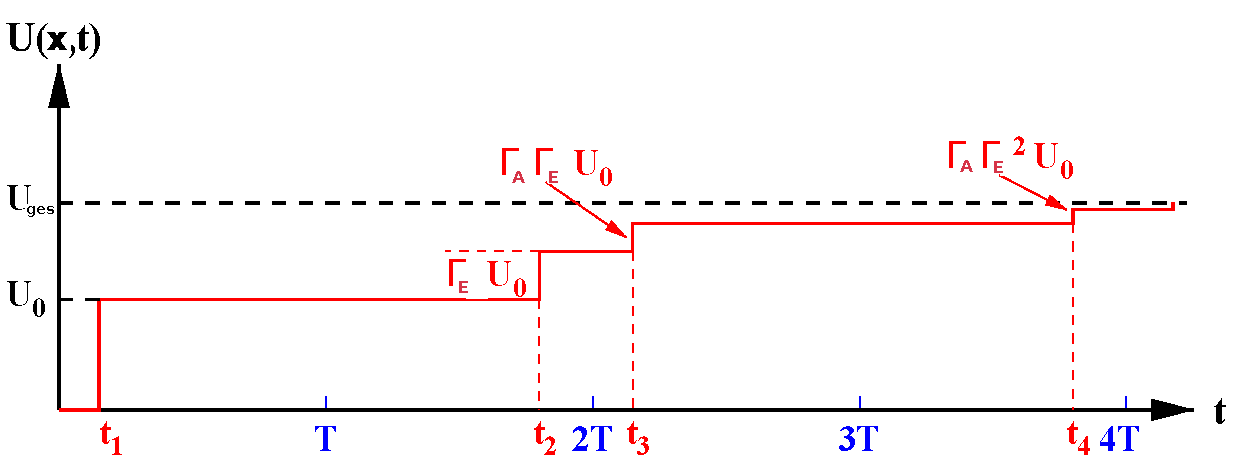
\includegraphics[width=0.6\textwidth]{Verlauf.pdf}
	\caption[Zeitlicher Verlauf der Signalspannung]{Zeitlicher Verlauf der Signalspannung $U(x,t)$ an einem festen Ort $x=ct_1$ \cite{E2}}
	\label{fig:ZeitlicherVerlauf}
\end{figure}

\subsection{Koaxialkabel}
Im Experiment werden Koaxialkabel verwendet. Sie bestehen aus zwei ineinander steckenden zylinderförmigen Leitern. Das Verhältnis der beiden Durchmesser bestimmt maßgeblich den Wellenwiderstand $Z_0$, den Längsspannungsverlust $R$ und den Querstromverlust $G$. Eine der Quellen dieser Verluste ist bei einem Koaxialkabel der \textit{Skin-Effekt}, d.h. das Verdrängen des Stroms aus dem Leiterinneren nach außen. Er wird dadurch verursacht, dass sich im Inneren des Leiters durch die Wechselspannung Wirbelfelder ausbilden, die den Wechselstrom wiederum nach außen verdrängen. Dieser Effekt ist bei hohen Frequenzen stärker, sodass $R$ und $G$ bei über \SI{100}{\kilo\hertz} nicht mehr frequenzunabhängig sind, sondern mit $\sqrt{\omega}$ ansteigen. \\
Für die Leitungskonstanten eines Koaxialkabels gelten die folgenden Beziehungen:
\begin{align}\label{eq:Theorie}
	R &= \frac{\sqrt{\frac{\pi\nu\mu_c}{\omega\Im{\varepsilon}}}}{2\pi}\left(\frac{1}{d}+\frac{1}{D}\right) \\
	&= \frac{\sqrt{\pi\rho\mu f}}{\pi}\left(\frac{1}{d}+\frac{1}{D}\right) \text{Die ist aus einer Quelle im Internet.} \\
	&= \sqrt{\frac{\mu f}{\sigma\pi}}\left(\frac{1}{d}+\frac{1}{D}\right) \\
	L &= \frac{\mu}{2\pi}\ln(\frac{D}{d}) \\
	G &= \frac{2\pi\sigma}{\ln(\frac{D}{d})} \\
	C &= \frac{2\pi\varepsilon}{\ln(\frac{D}{d})}
\end{align}
Hierbei sind $\varepsilon$ die Permittivität, $\mu$ die Permeabilität, $\sigma$ die spezifische Leitfähigkeit und $\rho$ der spezifische Widerstand.
\begin{figure}[h]
	\centering
	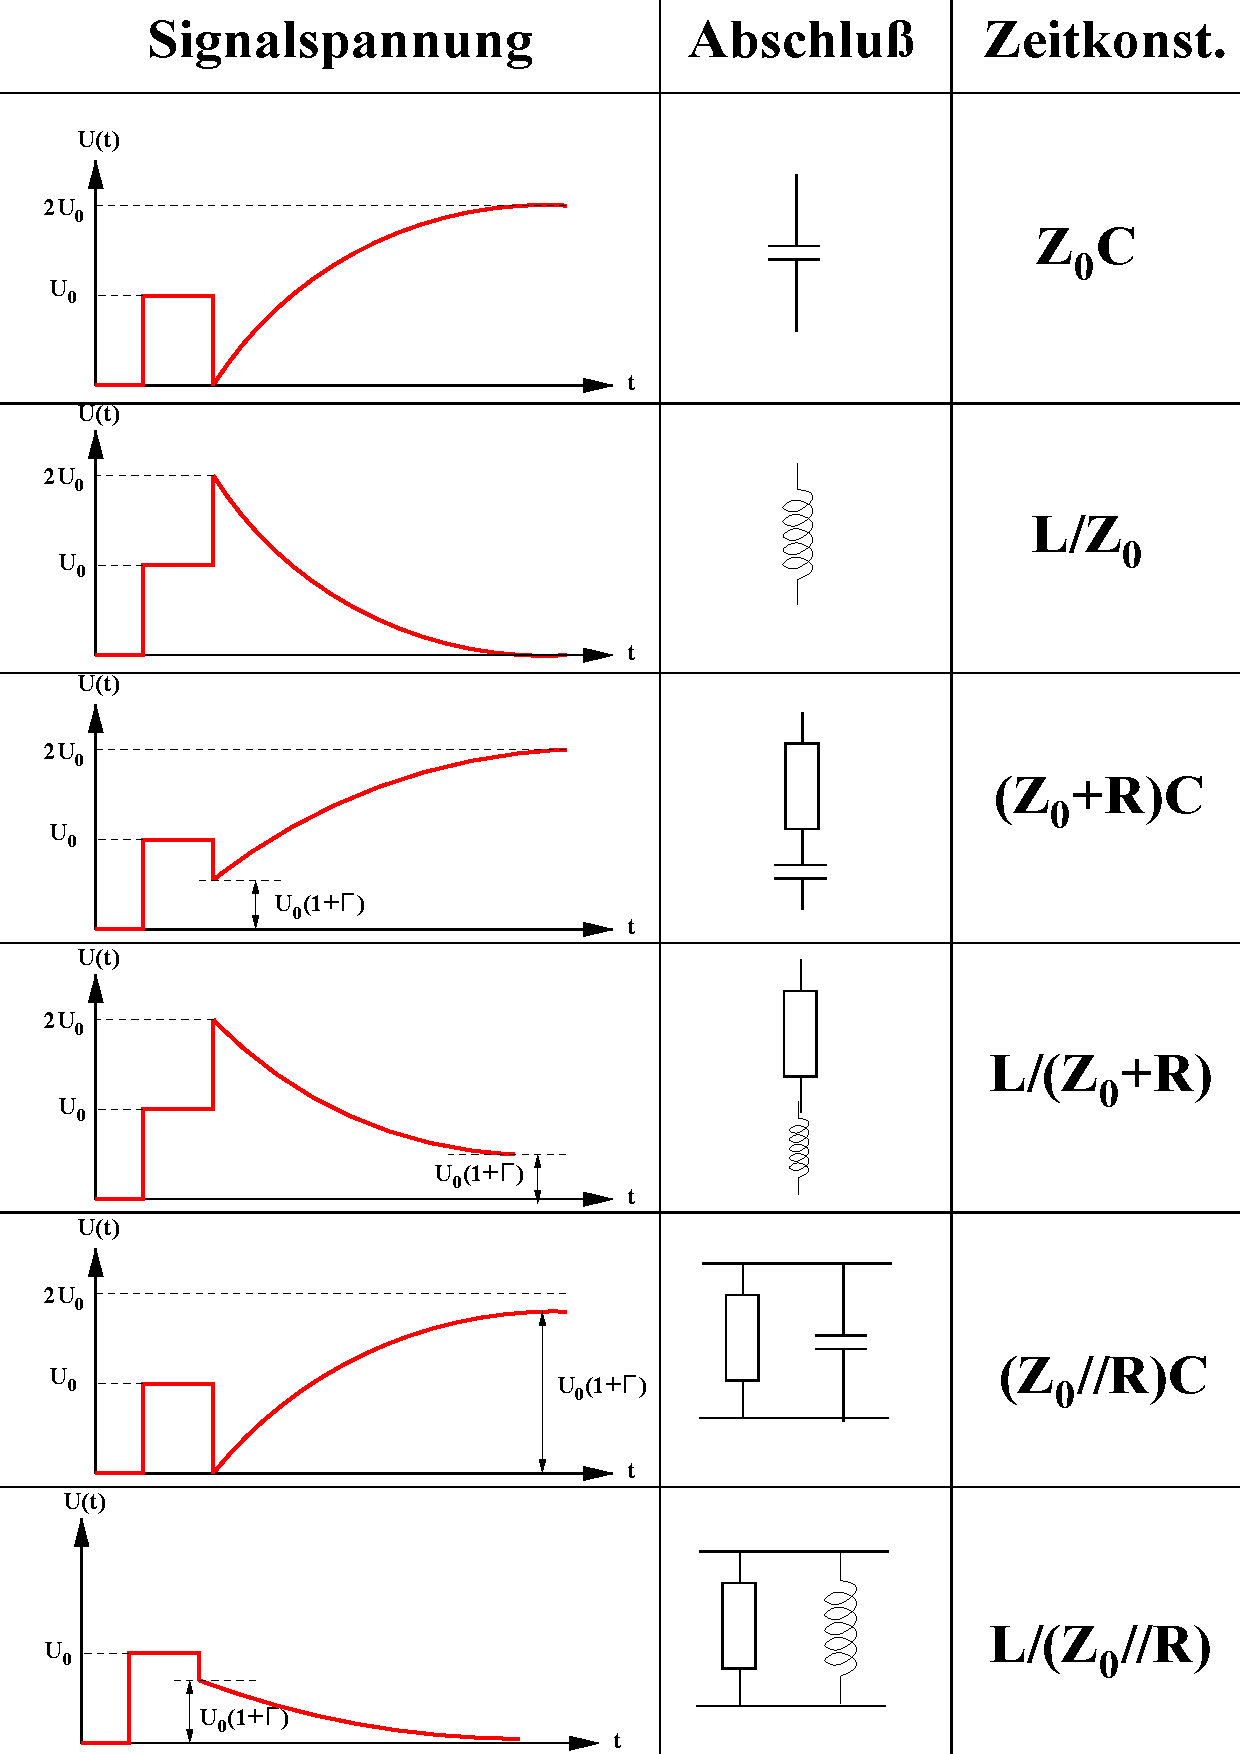
\includegraphics[width=0.55\textwidth]{Zeitkonstante.pdf}
	\caption{Signalspannung $U(x,t)$ und Zeitkonstanten für verschiedene Abschlusswiderstände \cite{E2}}
	\label{fig:Zeitkonstanten}
\end{figure}
\subsection{Laplace-Transformationen}\todo{evtl. auch in den Anhang oder woanders hin}
Eingangsspannung: $U_0\cdot\theta(t)\rightarrow U_h(p) = \frac{U_0}{p}$ \\
$LR$: $Z_A(t) = R + i\omega L$, $Z_A(p) = R + pL$.
\begin{align*}
	U_\text{RL}(t) &= U_0 + U_\text{r}(t) \\
	&= U_0 + \mathcal{L}^{-1}\left(\frac{Z_A(p)-Z_0}{Z_A(p)+Z_0}\frac{U_0}{p}\right) \\
	???? &= U_0 + \frac{R-Z_0}{R+Z_0}U_0\mathcal{L}^{-1}\left(\frac{1}{p}\right) + \frac{2Z_0L}{R+Z_0}U_0\mathcal{L}\left(\frac{1}{pL+R+Z_0}\right) \\
	&= U_0 + \frac{R-Z_0}{R+Z_0}U_0 + \frac{2Z_0L}{R+Z_0}U_0\exp\left(-\frac{R+Z_0}{L}t\right) \\
	&= U_0\left(1 + \frac{R}{R+Z_0} - \frac{Z_0}{R+Z_0} + \frac{2Z_0L}{R+Z_0}\exp\left(-\frac{R+Z_0}{L}t\right)\right)
\end{align*}
Bei Leanna kommt in der letzten Zeile was anderes raus...
\clearpage


\section{Aufbau und Ablauf des Experiments}
In diesem Kapitel wird zunächst die Hochfrequenzmethode zur Bestimmung der Energiedifferenz erklärt und dann das konkrete Vorgehen bei der Versuchsdurchführung.

\subsection{Hochfrequenzmethode}
Nachdem sich die Besetzungsinversion eingestellt hat, gibt es zwei verschiedene Arten, wie die Elektronen zurück in den Grundzustand gelangen können. Dies sind die spontane Emission und die induzierte Emission, die durch anregende Photonen mit einer Energie, die genau die der Energiedifferenz entspricht, erfolgt
\begin{align}\label{eq:Resonanz}
	h\nu = g_F\mu_\text{B}B_m \quad .
\end{align}
Welche Art der Emission dominiert hängt im wesentlichen von der Frequenz des Abstrahlvorgangs ab. In unserem Fall treten fast ausschließlich induzierte Emissionen auf. Um die Breite der Energielücke zu bestimmen sucht man die Resonanzstelle. \\
\begin{figure}[H]
	\centering
	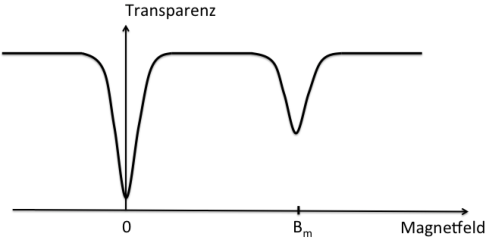
\includegraphics[width=0.6\textwidth]{Abb10.pdf}
	\caption[Transparenz]{Transparenz des Alkali-Gases in einem von außen angelegtem Magnetfeld, um die Resonanzfrequenz zu treffen \cite{\V}}
	\label{fig:transparenz}
\end{figure}
Die Resonanzstelle kann gut durch die Transparenz des Gases gefunden werden (siehe Abb. \ref{fig:transparenz}). Das Gas wird permanent mit rechtszirkular polarisiertem Licht bestrahlt. Ab dem Moment wenn die Besetzungsinversion einsetzt, ist das Gas transparent. Wenn nun die induzierte Emission eintritt, ist das Grundniveau wieder besetzt und das einfallende Licht hebt die Elektronen auf einen höheren Zustand. Das Gas ist nicht mehr vollständig transparent. Das Gas erreicht diesen Zustand jedoch bald wieder.\\
Der Versuchsaufbau, um die Resonanzen zu finden ist in Abb. \ref{fig:aufbau} dargestellt. Die Spektrallampe liefert das Licht, um die Elektronen anzuregen. Das Licht wird in einem Polarisator rechtszirkular polarisiert und mit einer Sammellinse auf das Alkali-Gas aus Rubidium 85 und Rubidium 87 Isotopen fokussiert. Das erhitzte Alkali-Gas befindet sich im thermodynamischen Gleichgewicht. Der Kolben ist von drei Holmholtz-Spulen umgeben und einer Spule, die die Hochfrequenz generiert. Die Frequenz wird immer auf einen festen Wert zwischen \si{100}{\kilo\hertz} und \si{1}{\mega\hertz} eingestellt und das Magnetfeld fährt einen Bereich kontinuierlich durch (Modulationsfeldspule). Auf der anderen Seite des Kolbens ist eine Diode, die an ein Oszilloskop angeschlossen ist. 
\begin{figure}[H]
	\centering
	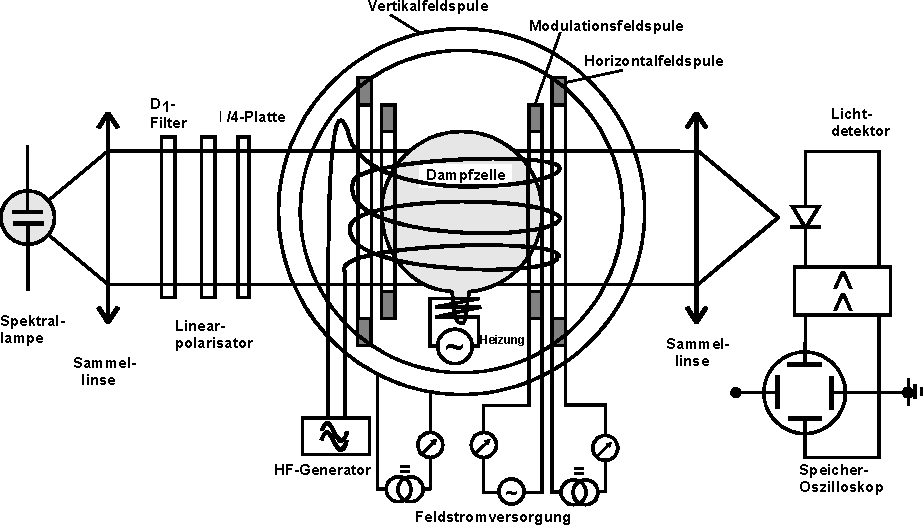
\includegraphics[width=\textwidth]{Abb13.pdf}
	\caption{Versuchsaufbau \cite{\V}}
	\label{fig:aufbau}
\end{figure}


\subsection{Durchführung}
Insgesamt wird eine Messreihe und ein Bild aufgenommen. In der Messreihe werden die Frequenzen und Magnetfelder an der Resonanzstelle der beiden verschiedenen Isotope aufgenommen. Das Bild zeigt den Spannungsverlauf am Oszilloskop, der die typische Transparenzkurve darstellt. Die einzelnen Schritte der Vorbereitung und der Messung sind folgende:
\begin{enumerate}
	\item Der Strahlengang wird durch die Sammellinsen so aufgebaut, dass das die Diode eine maximale Spannung ausgibt. 
	\item Das Magnetfeld wird berücksichtigt. Die horizontale Komponente wird durch Drehen des gesamten Aufbaus verändert und die vertikale durch die vertikale Helmholtz-Spule. Beides wird so eingestellt, dass die ansteigende Flanke der Transparenz-Kurve möglichst steil ist. 
	\item Für den Frequenzbereich \si{100}{\kilo\hertz} bis \si{1}{\mega\hertz} wird in Abständen von \si{100}{\kilo\hertz} die Resonanzstelle beider Isotope gesucht. Dafür verwendet man die Modulationsfeldspule. Reicht der Bereich der Modulationsfeldspule nicht aus, wird zusätzlich ein Magnetfeld durch die horizontale Helmhotz-Spule angelegt.
	\item Ein Bild eines typischen Signalverlaufs soll aufgenommen werden.
\end{enumerate}



\clearpage


\section{Auswertung}
\todo{Die Mehrfachreflexion sollte zuerst kommen, da ich mir hier einen Weg zur Berechnung der Kabellänge überlegt habe. Leanna hatte dazu ne extra Messung, wir nicht. Du kannst ja mal schauen, ob der Weg für dich so Sinn macht.}
\todo[color=green]{Ich finde die Methode logisch - mir gefällt sie :-), aber was ist dein v?}
\subsection{Mehrfachreflexion}
\subsubsection{Impulsfahrplan}
Abbildung \ref{fig:Impulsfahrplan} zeigt den Impulsfahrplan für die betrachtete Mehrfachreflexion, sie ist nicht Maßstabsgetreu. Die breiten Linien kennzeichnen, dass hier zwei verschiedene Impulse überlagert werden. Es wird angenommen, dass die Verbindung von Kabel 1 zum Oszilloskop perfekt transmittierend ist, d.h. $\Gamma_A = 0$. Die Reflexionen, die dann noch übrig sind, sind in rot gezeichnet.
\begin{figure}[h]
	\centering
	\begin{tikzpicture}
	\draw[line width=2pt] (0,0) -- (0,10);
	\draw[line width=2pt] (11,0) -- (11,10);
	\draw[line width=2pt] (5,0) -- (5,10);
	\draw[->] (-0.5,0) -- node [yshift = 5.5cm]{$t$} (-0.5,10.5);
	\draw[->] (-0.5,0) -- node [xshift = 6.5cm]{$x$} (11.5,0);
	% Linie1
	\draw (0,0) -- (11,1/5*11);
	\draw (11,1/5*11) -- (0,1/5*11*2);
	\draw (0,1/5*11*2) -- (11,1/5*11*3);

	% Linie2
	\draw (5,1) -- (0,2);
	\draw (0,2) -- (11,1/5*11+2);
	\draw (11,1/5*11+2) -- (0,1/5*11*2+2);
	\draw (0,1/5*11*2+2) -- (11,1/5*11*3+2);
	
	%Linie3
	\draw (5,3) -- (0,4);
	\draw (0,4) -- (11, 1/5*11+4);
%	\draw (11, 1/5*11+4) -- (0,1/5*11*2+4);
	
	%Linie4
	\draw (5,5) -- (0,6);
	\draw (0,6) -- (11,1/5*11+6);
	
	\draw (5,1/5*11*2-1) -- (11,1/5*11*2-1+1/5*6);
	\draw (11,1/5*11*2-1+1/5*6) -- (0,1/5*11*2-1+1/5*6+1/5*11);
	\draw (0,1/5*11*2-1+1/5*6+1/5*11) -- (11,1/5*11*2-1+1/5*6+1/5*11*2);
\end{tikzpicture} \\
	\caption[Impulsfahrplan]{Impulsfahrplan zur Veranschaulichung der Mehrfachreflexion}
	\label{fig:Impulsfahrplan}
\end{figure}
%\clearpage
\subsubsection{Bestimmung der Reflexionskonstanten}
Das am Oszilloskop aufgenommene Bild ist in Abbildung \ref{fig:Mehrfachreflexion} zu sehen. Es sind vier Plateaus, $U_0,U_1,U_2,U_3$, erkennbar. Um sie zu berechnen werden die in Abbildung \ref{fig:U} jeweils farbig markierten Werte verwendet und gemittelt. Die gestrichelten Linien zeigen die daraus erhaltenen Mittelwerte
\begin{align}
	U_0 &= \SI{-1.81994+-0.00002}{\kilo\volt}
 \notag \\
	U_1 &= \SI{-1.1}{\kilo\volt}
 \notag \\
	U_2 &= \SI{119.04+-0.03}{\volt}
 \notag \\
	U_3 &= \SI{-0.4}{\kilo\volt}
  \ .
\end{align}
Die Spannungsdifferenzen $\Delta U_i = U_i-U_{i-1}$ können im Impulsfahrplan abgelesen werden:
\begin{align}
	\Delta U_1 &= \Gamma_{12}U_0 \notag \\
	\Delta U_2 &= (1-\Gamma_{21})\Gamma_E(1-\Gamma_{12})U_0 \notag \\
	\Delta U_3 &= (1-\Gamma_{21})\Gamma_E^2\Gamma_{21}(1-\Gamma_{12})U_0 \quad.
\end{align}
Die Lösung dieses Gleichungssystems ergibt die Reflexionskonstanten
\begin{align}
	\Gamma_{12} &= \frac{\Delta U_1}{U_0} &&= \SI{0.4}{}
\notag \\
	\Gamma_{21} &= \frac{1}{1+\frac{\Delta U_2^2}{\Delta U_3(U_0-\Delta U_1)}} &&= \SI{1.0}{}
\notag \\
	\Gamma_E &= \frac{\Delta U_3}{\Delta U_2} + \frac{\Delta U_2}{U_0-\Delta U_1} &&= \SI{4.872+-0.001}{}
\notag \quad,
\end{align}\todo{Was zur Hölle sind das für Werte?}
wobei $\Gamma_E \not= 0$ und $\Delta U_1 \not= U_0$ gelten muss.

\begin{figure}[h]
	\centering
	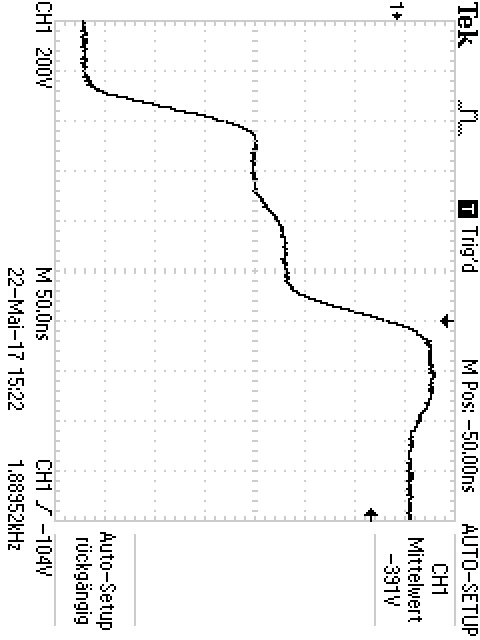
\includegraphics[width=0.6\textwidth]{Oszilloskop/Mehrfachreflexion/F0054TEK.JPG}
	\caption[Mehrfachreflexion]{Bild am Oszilloskop bei der Mehrfachreflexion}
	\label{fig:Mehrfachreflexion}
\end{figure}
\begin{figure}[h]
	\centering
	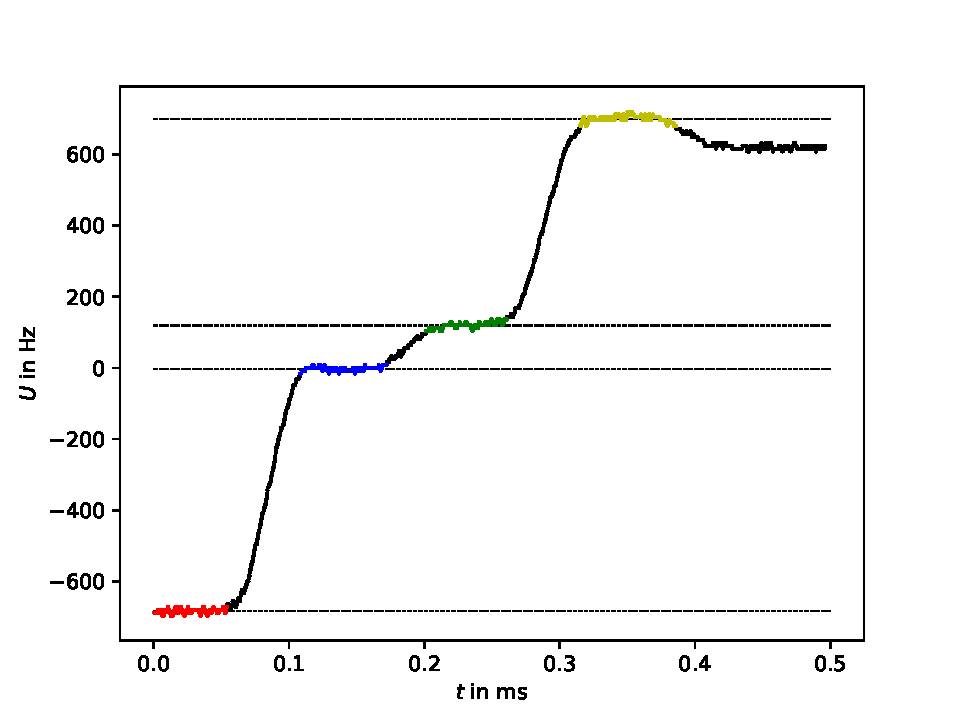
\includegraphics[width=0.7\textwidth]{Plot.pdf}
	\caption{Veranschaulichung der Messdaten aus dem Oszilloskop-Bild und der berechneten Plateau-Spannungen}
	\label{fig:U}
\end{figure}
\subsubsection{Bestimmung der Kabellängen}
$T$ ist die Zeit zwischen zwei Signalen. Der Beginn eines Signals wird als der Beginn des Plateaus definiert. Damit gilt
\begin{align}
	T_1 &= \SI{0.108}{\micro\second}
 \notag \\
	T_2 &= \SI{0.093}{\micro\second}
 \notag \\
	T_3 &= \SI{0.114}{\micro\second}
 \quad.
\end{align}
Es gelten die Beziehungen (siehe Impulsfahrplan \ref{fig:Impulsfahrplan})
\begin{align*}
	T_1 &= \frac{2L_1}{v} \\
	T_2 &= \frac{2L_1 + 2L_2}{v}-T_1 = \frac{2L_2}{v} \\
	T_3 &= \frac{2L_1+4L_2}{v}-T_2 = \frac{2L_2}{v} \quad.
\end{align*}
Die Geschwindigkeit ist der Quotient aus der Vakuumlichtgeschwindigkeit und der Wurzel der relativen Permittivität von Kupfer. Nach den Längen aufgelöst ergibt sich so
\begin{align}
	L_1 &= \SI{10.8}{\meter}
 \notag \\
	L_2 &= \SI{10.3+-0.7}{\meter}
 \quad, 
\end{align}
wobei $L_2$ einmal mit $T_2$ und einmal mit $T_3$ ausgerechnet wurde und hier der Mittelwert steht.\clearpage
\subsection{Leitungskonstanten direkt}
Die gemessenen Werte für $R,C,L$ für die beiden Kabel stehen in den Tabellen \ref{tab:RLC50Werte} und \ref{tab:RLC75Werte}. Die Werte für $G$ werden berechnet, indem
eine verzerrungsfreie Übertragung angenommen wird, d.h. der Phasenbelag $k$ aus \eqref{eq:LosungTelegraph} muss verschwinden. Daraus ergibt sich die Bedingung
\begin{align}
	G = -\frac{RL}{C} \quad.
\end{align}
Mit Hilfe von \eqref{eq:RLCTheorie} können folgende theoretische Vergleichswerte ausgerechnet werden
\begin{align}
	R &= \SI{122.6}{\micro\ohm\per\meter}
 \notag \\
	C &= \SI{105.4}{\pico\farad\per\meter}
 \notag \\
	L &= \SI{237.4}{\nano\farad\per\meter}
 \notag \\
	G &= \SI{54.4}{\nano\siemens\per\meter}
 \quad,
\end{align}
die zusammen mit den Messwerten in den Abbildungen \ref{fig:PlotR} - \ref{fig:PlotG} abgebildet sind.
\begin{table}
    \centering
    \caption{Beim Kurzschließen des $50\Omega$-Kables gemessene Werte für $R_{50},C_{50},L_{50}$ und daruas berechnete Werte für $G_{50}$ bei den jeweils eingestellten Frequenzen $f$}
    \label{tab:RLC50Werte}
    \sisetup{parse-numbers=false}
    \begin{tabular}{
	S[table-format=3.1]
	S[table-format=1.4]
	S[table-format=3.1]
	S[table-format=1.2]
	S[table-format=1.1]
	}
	\toprule
	{$f_{50} \ \mathrm{in} \ \si{\kilo\hertz}$}		& {$R_{50} \ \mathrm{in} \ \si{\ohm}$}		& 
	{$C_{50} \ \mathrm{in} \ \si{\pico\farad}$}		& {$L_{50} \ \mathrm{in} \ \si{\micro\henry}$}		& 
	{$G_{50} \ \mathrm{in} \ \si{\milli\siemens}$}		\\ 
	\midrule
    \input{RLC_DirekteMessung/build/tableRLC50.tex}
    \bottomrule
    \end{tabular}
    \end{table}

\begin{table}
    \centering
    \caption{Beim Kurzschließen des $75\Omega$-Kables gemessene Werte für $R_{75},C_{75},L_{75}$ und daraus berechnete Werte für $G_{75}$ bei den jeweils eingestellten Frequenzen $f$}
    \label{tab:RLC75Werte}
    \sisetup{parse-numbers=false}
    \begin{tabular}{
	S[table-format=3.0]
	S[table-format=1.2]
	S[table-format=3.1]
	S[table-format=1.2]
	S[table-format=1.1]
	}
	\toprule
	{$f_{75} \ \mathrm{in} \ \si{\kilo\hertz}$}		& {$R_{75} \ \mathrm{in} \ \si{\ohm}$}		& 
	{$C_{75} \ \mathrm{in} \ \si{\pico\farad}$}		& {$L_{75} \ \mathrm{in} \ \si{\micro\henry}$}		& 
	{$G_{75} \ \mathrm{in} \ \si{\milli\siemens}$}		\\ 
	\midrule
    \input{RLC_DirekteMessung/build/tableRLC75.tex}
    \bottomrule
    \end{tabular}
    \end{table}

\begin{figure}[h]
	\centering
	\begin{subfigure}{0.496\textwidth}
		\centering
		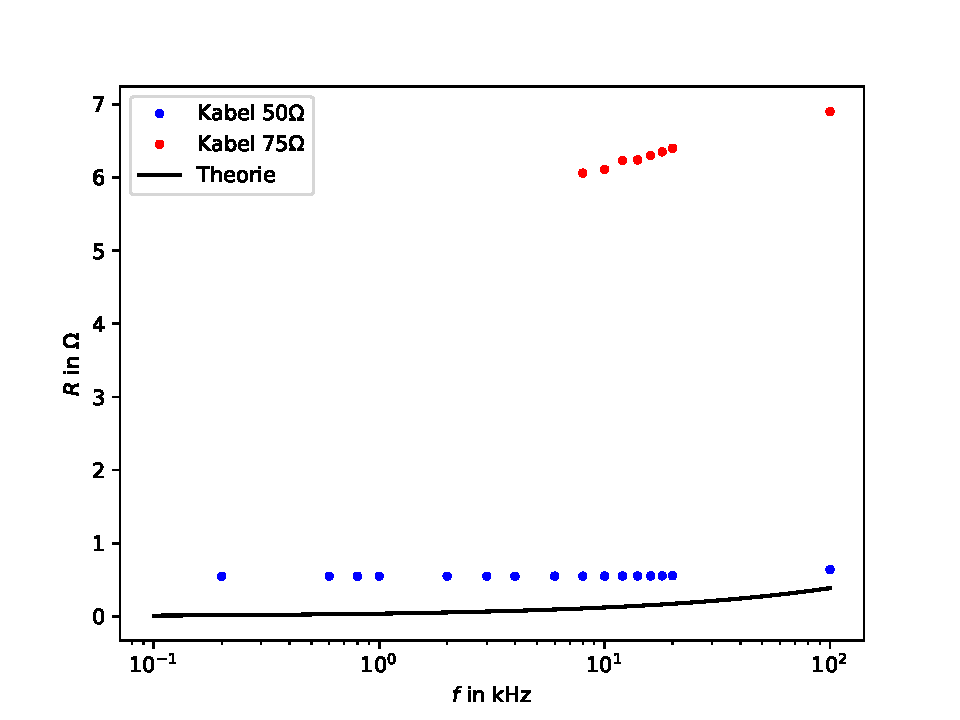
\includegraphics[width=\textwidth]{RLC_DirekteMessung/build/PlotR.pdf}
		\subcaption{Werte für $R$}
		\label{fig:PlotR}
	\end{subfigure}
	\begin{subfigure}{0.496\textwidth}
		\centering
		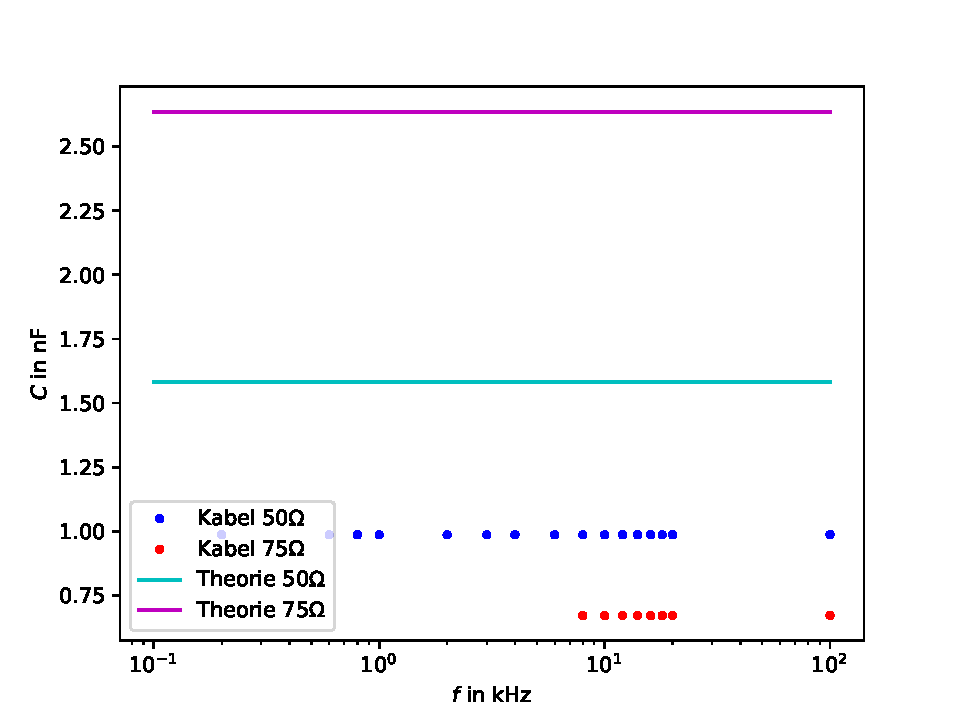
\includegraphics[width=\textwidth]{RLC_DirekteMessung/build/PlotC.pdf}
		\subcaption{Werte für $C$}
		\label{fig:PlotC}
	\end{subfigure}
	\begin{subfigure}{0.496\textwidth}
		\centering
		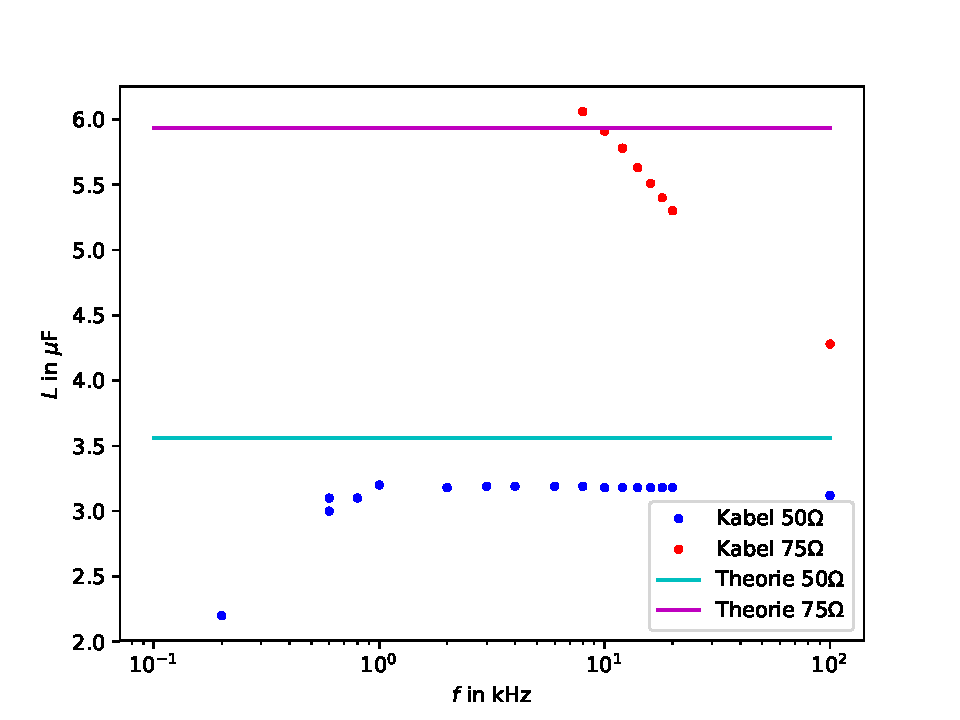
\includegraphics[width=\textwidth]{RLC_DirekteMessung/build/PlotL.pdf}
		\caption{Werte für $L$}
		\label{fig:PlotL}
	\end{subfigure}
	\begin{subfigure}{0.496\textwidth}
		\centering
		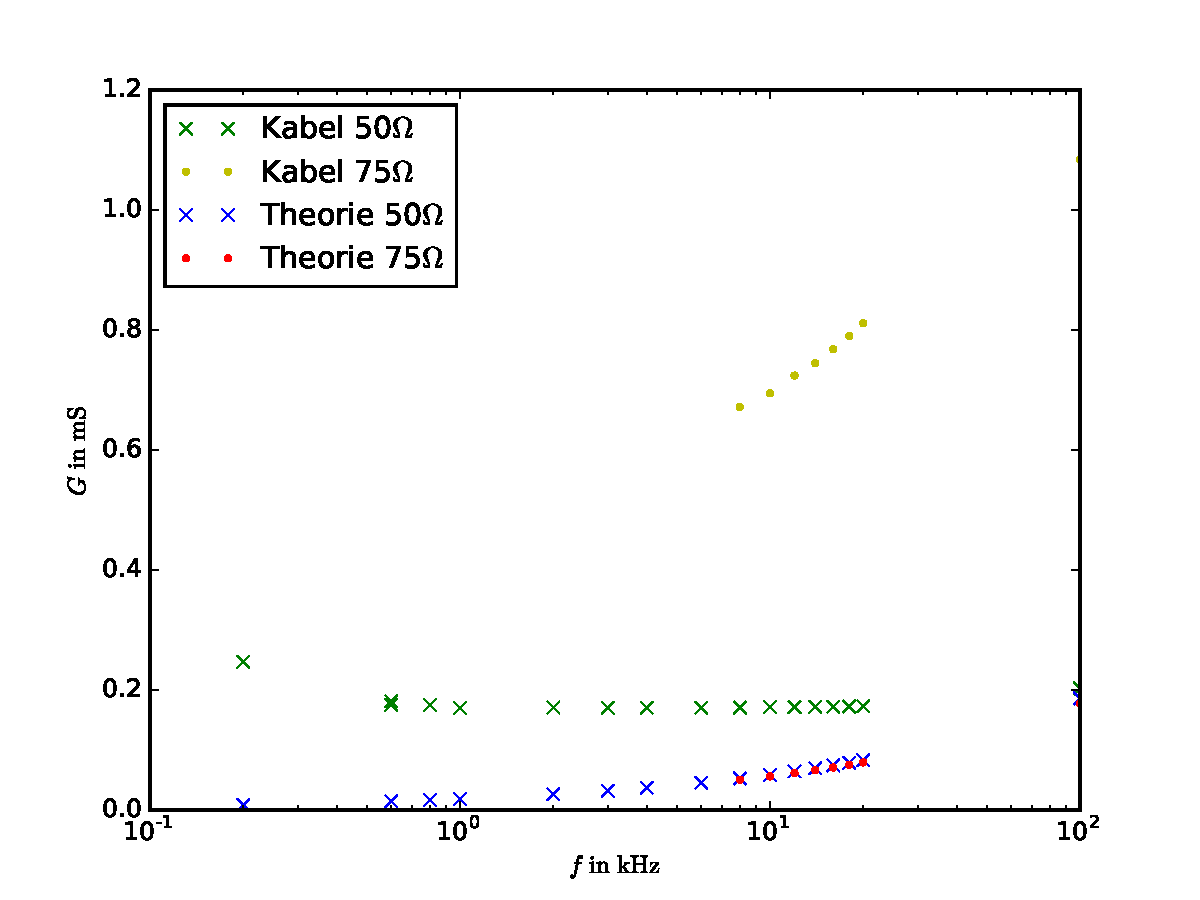
\includegraphics[width=\textwidth]{RLC_DirekteMessung/build/PlotG.pdf}
		\caption{Werte für $G$}
		\label{fig:PlotG}
	\end{subfigure}
	\caption[Werte bei der direkten Messung]{Gemessene Werte für $R,C,L$ bei der direkten Messung, sowie Theoriewerte und berechnete Werte für $G$}
	\label{fig:PlotRLCG}
\end{figure}\clearpage
\subsection{Leitungskonstanten R, L, C -- Signalverlauf}
Die Signalverläufe geben Aufschluss über die Leitungskonstanten der Kabel. Wie in Kapitel \ref{seq:laplace} gezeigt, entstehen unterschiedliche Spannungsverläufe für unterschiedliche Ausgangsimpedanzen. Das geschlossene Kabel entspricht einer Induktivität und das offene Kabel einer Kapazität. Als Impedanz $Z_0$ ist für das vermessene Kabel ist
\begin{equation}
	Z_0 = \si{50}{\ohm}
\end{equation}
angegeben. Der Spannungsverlauf wird mit einem Oszilloskop aufgezeichnet und die Werte an den theoretischen Verlauf der Kurve gefittet.

\subsubsection{Kabel mit geschlossenem Ende}
Der Signalverlauf ist in Abb. \ref{fig:oszi_geschlossen} dargestellt. Erwartet wird eine Flanke der Form
\begin{align}
			U(t) &= 2U_0\left(1 - \frac{Z_0}{R+Z_0} + \frac{Z_0}{R+Z_0}\exp\left(-\frac{R+Z_0}{L}t\right)\right) \\
			&= 2 a \left(1- b + b \exp(-c (t+d))   \right) + e \quad .
\end{align}
Es ist nur mit einer geeigneten Wahl der Startparameter möglich, einen guten Fit zu bekommen. Leider sind die so erhaltenen Abweichungen der Parameter dann unrealistisch und werden deswegen nicht weiter betrachtet. Die Funktion ist in Abb. \ref{fig:fit_geschlossen} dargestellt. Die verwendeten Parameter sind:
\begin{align}
	a &= \SI{-6.7339}{\volt}
 \\
	b &= \SI{0.9872}{}
 \\
	c &= \SI{0.0089}{\ohm\per\henry}
 \\
	d &= \SI{483.2099}{\nano\second}
 \\
	e &= \SI{12.5272}{\volt}
 
\end{align}
Aus den Parametern können der Widerstandsbelag $R$ und der Induktivitätsbelag $L$ des Kabels berechnet werden. Es muss beachtet werden, dass die Zeitskala Nanosekunden ist.
\begin{align}
	R &= \frac{Z_0}{b} - Z_0 = \SI{0.6507}{\ohm}
 \\
	L &= \frac{R + Z_0}{ c \cdot 10^9} = \SI{5.6828}{\micro\henry}

\end{align}



\begin{figure}
	\centering
	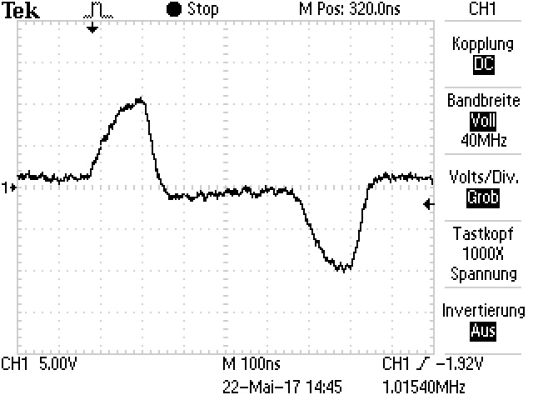
\includegraphics[width=0.7\textwidth]{Laplace/geschlossen.pdf}
\caption{Spannungsverlauf bei dem Kabel mit geschlossenem Ende}
\label{fig:oszi_geschlossen}
\end{figure}

\begin{figure}
	\centering
	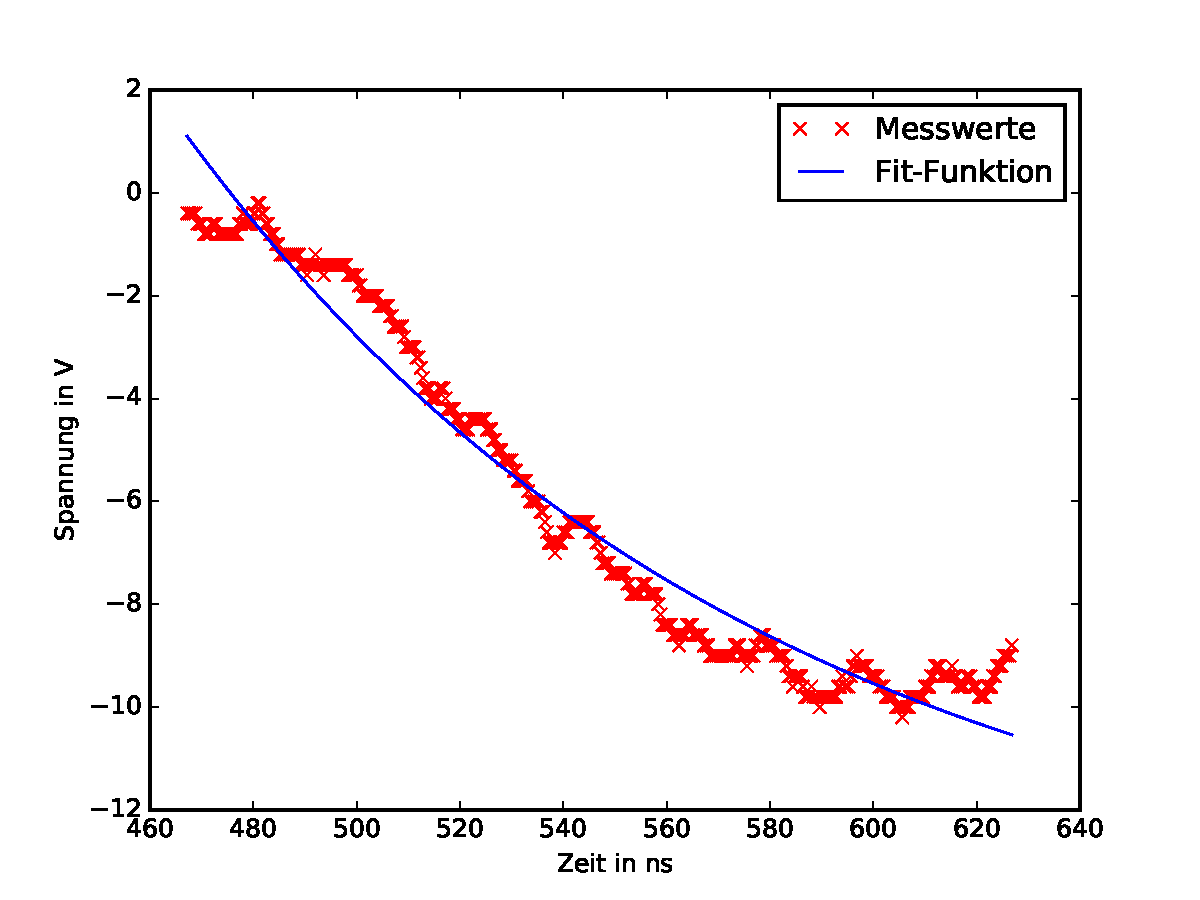
\includegraphics[width=0.7\textwidth]{Laplace/geschlossenes_ende.pdf}
	\caption{Fitfunktion an die fallende Flanke des Signalverlaufs bei dem Kabel mit geschlossenem Ende}
\label{fig:fit_geschlossen}
\end{figure}

\clearpage
\subsubsection{Kabel mit offenem Ende}
Der Spannungsverlauf des offenen Kabels ist in  Abb. \ref{fig:oszi_offen} zu sehen. Der Verlauf folgt der Funktionsvorschrift
\begin{align}
	U_0(t) &= 2U_0\left(1 -  \frac{Z_0}{R+Z_0} \exp \left( - \frac{1}{C(R+Z_0)} t\right) \right)\\
	&=  2 a (1 - b \exp(-c (x-d))) + e \quad .
\end{align}
Wie schon bei dem Kabel mit geschlossenem Ende müssen die Startwerte für die Parameter des Fits sehr exakt gewählt werden. Auch die ausgegebenen Abweichungen sind abermals nicht brauchbar. Der Plot ist in Abb. \ref{fig:fit_offen} dargestellt. Die Parameter sind:

\begin{align}
		a &= \SI{4.1028}{\volt}
 \\
		b &= \SI{0.6497}{}
 \\
		c &= \SI{0.0132}{\per\farad\per\ohm}
 \\
		d &= \SI{-466.8082}{\nano\second}
 \\
		e &= \SI{-10.8431}{\volt}
 
\end{align}
Es lassen sich die Kapazität $C$ des Kabels ebenso die der Widerstand $R$ aus den Parametern berechnen 
\begin{align}
	R &= \frac{Z_0}{b} - Z_0 = \SI{26.9529}{\ohm}
 \\
	C &= \frac{1}{ c (r + Z_0) \cdot 10^9} = \SI{985.9779}{\pico\farad}
 \quad.
\end{align}

\clearpage

\begin{figure}
	\centering
	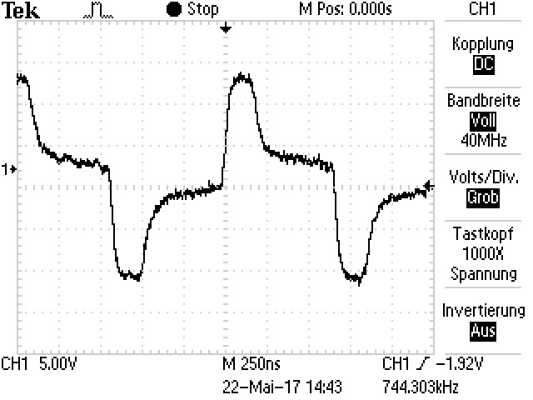
\includegraphics[width=0.7\textwidth]{Laplace/offen.pdf}
	\caption{Spannungsverlauf bei dem Kabel mit offenem Ende}
	\label{fig:oszi_offen}
\end{figure}

\begin{figure}
	\centering
	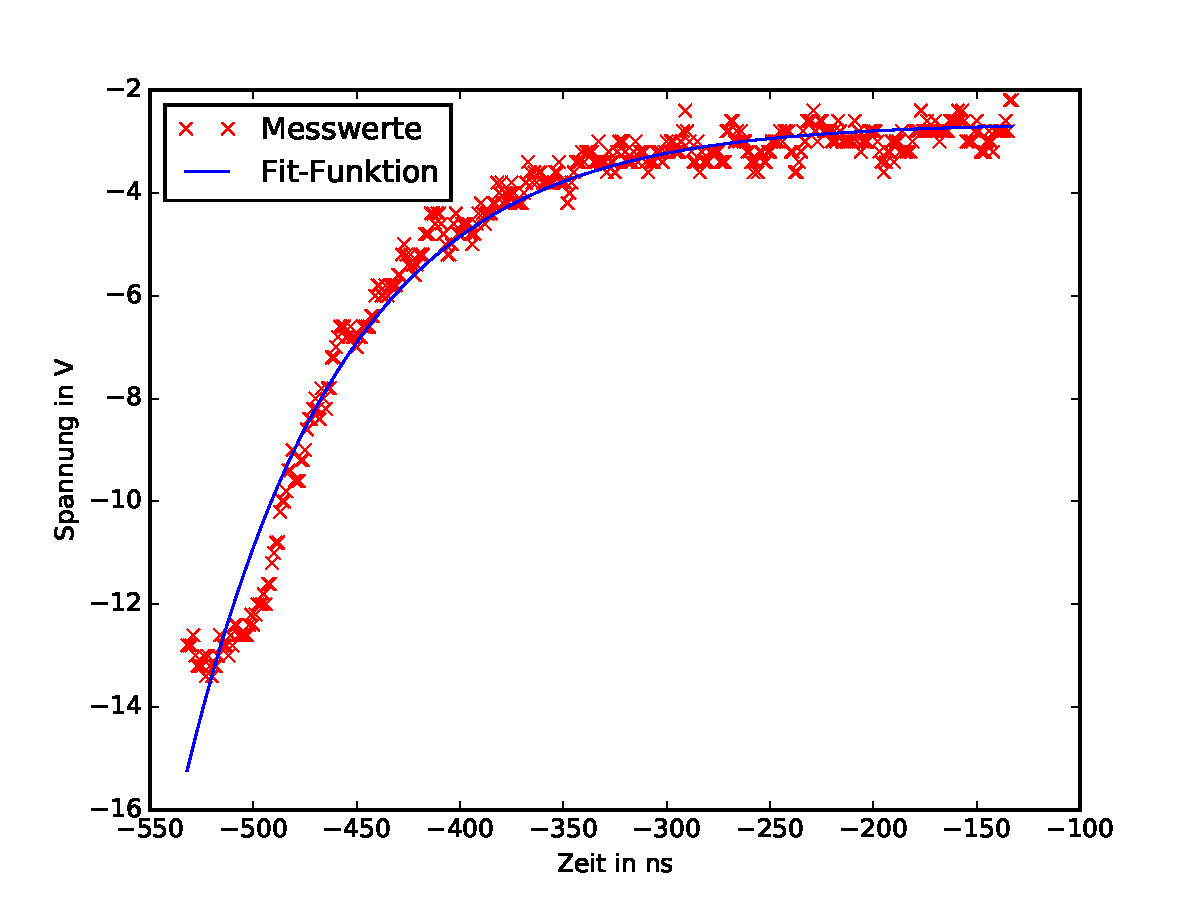
\includegraphics[width=0.7\textwidth]{Laplace/offenes_ende.pdf}
	\caption{Fitfunktion an die fallende Flanke des Signalverlaufs bei dem Kabel mit offenem Ende}
	\label{fig:fit_offen}
\end{figure}

\clearpage
\subsection{Leitungskonstanten durch Reflexion}
Offenes Ende: Form müsste RC-Parallelschaltung entsprechen. Rechne dafür die Laplace-Trafo aus. Fitte die ausgerechnete Funktion an die Werte. \\
Geschlossenes Ende: Form müsste LR-Reihenschaltung entsprechen. Rechne dafür die Laplace-Trafo aus. Fitte die ausgerechnete Funktion an die Werte.
\subsection{Dämpfungskonstante}
Zur Bestimmung der Dämpfungskonstante wird mit dem Oszilloskop für ein langes und ein kurzes Kabel eine FFT eines Rechteckpulses durchgeführt. Die hier entstandenen Bilder sind in Abbildung \ref{fig:FFT} zu sehen. Die Position und Höhe der Peaks wird aus dem Datensatz extrahiert und sind in Tabelle \ref{tab:DaempfungWerteB} zu sehen. \\
\begin{figure}[h]
	\centering
	\begin{subfigure}{0.495\textwidth}
		\centering
		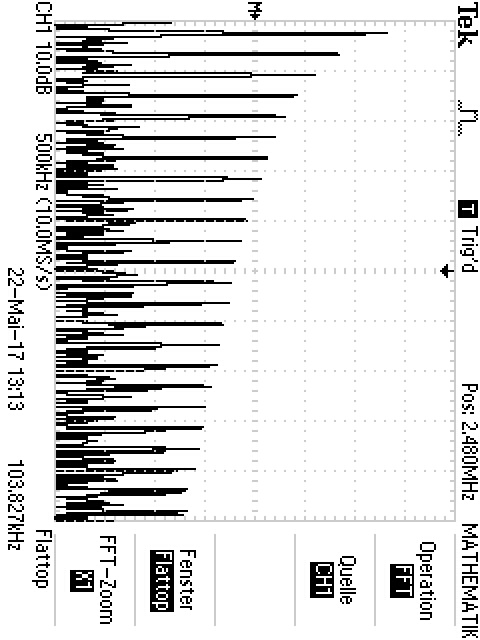
\includegraphics[width=0.9\textwidth]{Oszilloskop/DaempfungLang/F0042TEK.JPG}
		\subcaption{Langes Kabel}
		\label{fig:FFTLang}
	\end{subfigure}
	\begin{subfigure}{0.495\textwidth}
		\centering
		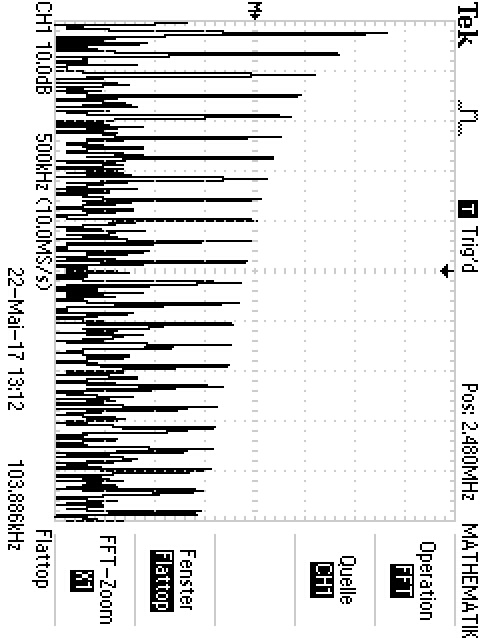
\includegraphics[width=0.9\textwidth]{Oszilloskop/DaempfungKurz/F0041TEK.JPG}
		\subcaption{Kurzes Kabel}
		\label{fig:FFTKurz}
	\end{subfigure}
	\caption{Oszilloskop-Bilder der FFT}
	\label{fig:FFT}
\end{figure}
Da ein ungerades Rechtecksignal betrachtet wird, sind die $\omega_n$ ungerade Vielfache der Grundfrequenz $\omega_0$. Es wird die Vermutung aufgestellt, dass das Oszilloskop die Fouriertransformierte dabei mit
\begin{align}\label{eq:Vermutung}
	P = \ln\left(\frac{U(\omega)}{U_0}\right)
\end{align}
normiert. Die Fourierkoeffizienten und die Fouriertransformierte eines ungeraden Rechtecksignals sind
\begin{align*}
	A_n &=\frac{4U_0}{\pi(2n+1)} = \frac{A_0}{2n+1} \quad, \\
	U(\omega) &= \sum_{n=0}^{\infty}A_n\delta(\omega-\omega_0(2n+1)) \quad.
\end{align*}
Die Amplituden, die das Oszilloskop mit der FFT darstellt können demnach auch durch die Fourierkoeffizienten ausgedrückt werden:
\begin{align}\label{eq:P}
	P_n = \ln\left(\frac{A_n}{A_0}\right) &= \ln\left(\frac{\omega_0}{\omega_n}\right)\notag \\
	&= \ln\left(\frac{\omega_0}{\omega_n}\right)\si{\neper}\notag \quad\footnotemark \\
	&= 20\log_{10}\left(\frac{\omega_0}{\omega_n}\right)\si{\deci\bel} \quad.
\end{align}
Die Grundfrequenz ist dabei
\begin{align*}
	\omega_0 = \frac{\omega(A_n)}{2n+1} = \input{Daempfung/build/omega0} \quad.
\end{align*}
Abbildung \ref{eq:DaempfungB} zeigt diese Amplituden zusammen mit den aus den Messwerten und bestätigt die Vermutung \eqref{eq:Vermutung}, wenn bedacht wird, dass auch beim kurzen Kabel Verluste z.B. an den Verbindungsstücken auftauchen. \footnotetext{\si{\neper} ist eine Einheit, die das Verhältnis von zwei Werten angibt. Sie kann hier einfach hinzugefügt werden, da \SI{1}{\neper} = 1.}
\begin{figure}[h]
	\centering
	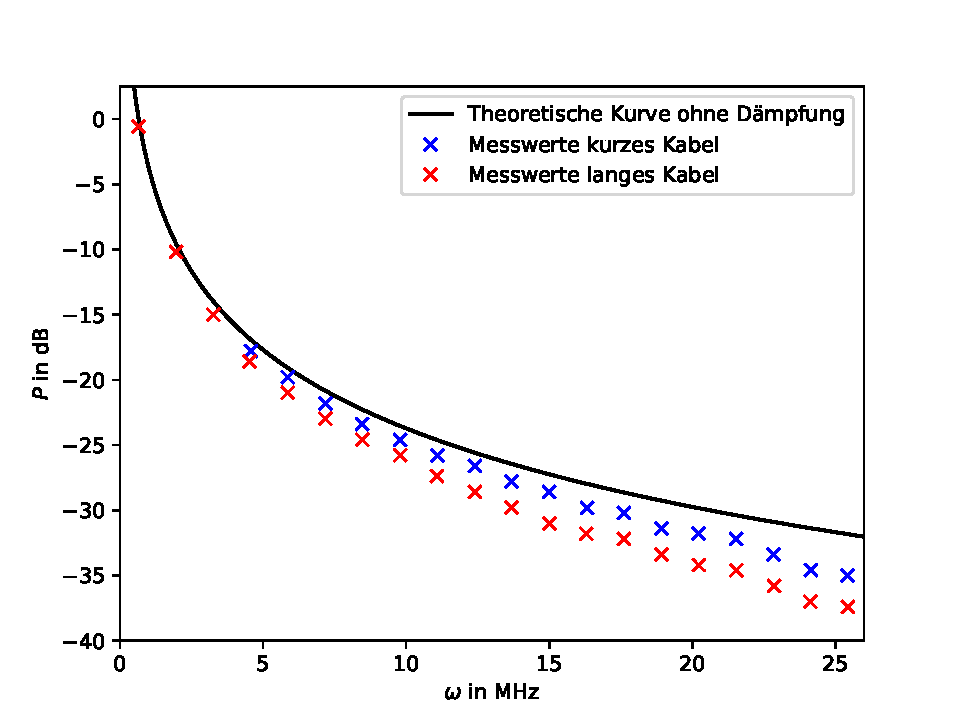
\includegraphics[width=0.8\textwidth]{Daempfung/build/PlotB.pdf}
	\caption{Aus dem Oszilloskop-Datensatz extrahierte Werte der Peaks mit der theoretischen Kurve aus \eqref{eq:P}}
	\label{fig:PlotDaempfungB}
\end{figure} \\
Die Dämpfungskonstante kann nun wie folgt berechnet werden
\begin{align}\label{eq:DaempfungB}
	P_{n,\text{Lang}}-P_{n,\text{Kurz}} &= \ln\left(\frac{U_{n,\text{Lang}}(\omega)}{U_0}\right) - \ln\left(\frac{U_{n,\text{Kurz}}(\omega)}{U_0}\right)\notag \\
	&= \ln\left(\frac{U_{n,\text{Lang}}(\omega)}{U_0}\right) - \ln\left(\frac{U_{n,\text{Kurz}}(\omega)}{U_0}\right)\si{\neper}\notag \\
	&= 20\cdot\log_{10}\left(\frac{U_{n,\text{Lang}}(\omega)}{U_{n,\text{Kurz}}(\omega)}\right)\si{\deci\bel}\notag \\
	&= 20\cdot\log_{10}\left(\exp(-\alpha L)\right)\si{\deci\bel}\notag \\
	&= -20\cdot\alpha\cdot L\cdot\log_{10}e\ \si{\deci\bel}\notag \\
	\Leftrightarrow\quad \alpha &= \frac{P_\text{Lang}-P_\text{Kurz}}{20\cdot L\cdot\log_{10}e\ \si{\deci\bel}} \quad.
\end{align}
Die  Werte für die Dämpfungskonstante sind in Tabelle \ref{tab:DaempfungWerteB} abgebildet. Die Mittelung ergibt
\begin{align}
	\alpha = \SI{3.64+-0.42}{\per\kilo\meter}
 \quad.
\end{align}
\begin{table}
    \centering
    \caption{Frequenz $\omega$ und Betrag der Amplitude $P$ der Peaks in der FFT für das kurze und das lange Kabel, sowie mit \eqref{eq:DaempfungB} berechnete Dämpfung}
    \label{tab:DaempfungWerteB}
    \sisetup{parse-numbers=false}
    \begin{tabular}{
	S[table-format=2.3]
	S[table-format=2.2]
	S[table-format=2.3]
	S[table-format=2.2]
	S[table-format=2.2]
	}
	\toprule
	{$\omega_\text{Kurz} \ \mathrm{in} \ \si{\mega\hertz}$}		& {$|P_\text{Kurz}| \ \mathrm{in} \ \si{\deci\bel}$}		& 
	{$\omega_\text{Lang} \ \mathrm{in} \ \si{\mega\hertz}$}		& {$|P_\text{Lang}| \ \mathrm{in} \ \si{\deci\bel}$}		& 
	{$\alpha \ \mathrm{in} \ \si{\per\kilo\meter}$}		\\ 
	\midrule
    \input{Daempfung/build/tableB.tex}
    \bottomrule
    \end{tabular}
    \end{table}


\subsection{Abschlussimpedanzen}
Das Koaxialkabel wird mit drei unterschiedlichen Abschlussimpedanzen versehen. Alle drei Impedanzen sollen bestimmt werden und je nach der Art der Impedanz die Kapazität~$C$ und Induktivität~$L$ sowie der Widerstand~$R$ bestimmt. Die Eingangsimpedanz ist weiterhin $Z_0 = \SI{50}{\ohm}$.

\subsubsection{Abschlussimpedanz 1}
Der Anzeige des Oszilloskops nach zu urteilen handelt es sich um einen Widerstand und einen Kondensator in Reihenschaltung. Es wird für die aufsteigende Flanke die selbe Fit-Funktion angelegt wie bereits in Kapitel \ref{sec:kapazitat}. Die Messwerte und die Funktion sind in Abb. \ref{fig:box25} dargestellt. Die Parameter sind:
\begin{align}
	a &= \SI{-12.6127}{\volt}
 \\
	b &= \SI{1.1270}{}
 \\
	c &= \SI{0.0017}{\per\farad\per\ohm}
 \\
	d &= \SI{-9.8317}{\nano\second}
 \\
	e &= \SI{1339.6486}{\volt}
 
\end{align}
Daraus ergibt sich für den Widerstand und die Kapazität:
\begin{align}
	R &= \frac{Z_0}{b} - Z_0 = \SI{18.3527}{\ohm}
 \\
	C &= \frac{1}{ c (r + Z_0) \cdot 10^9} = \SI{13241.8832}{\pico\farad}
 \quad.
\end{align}


\begin{figure}
	\centering
	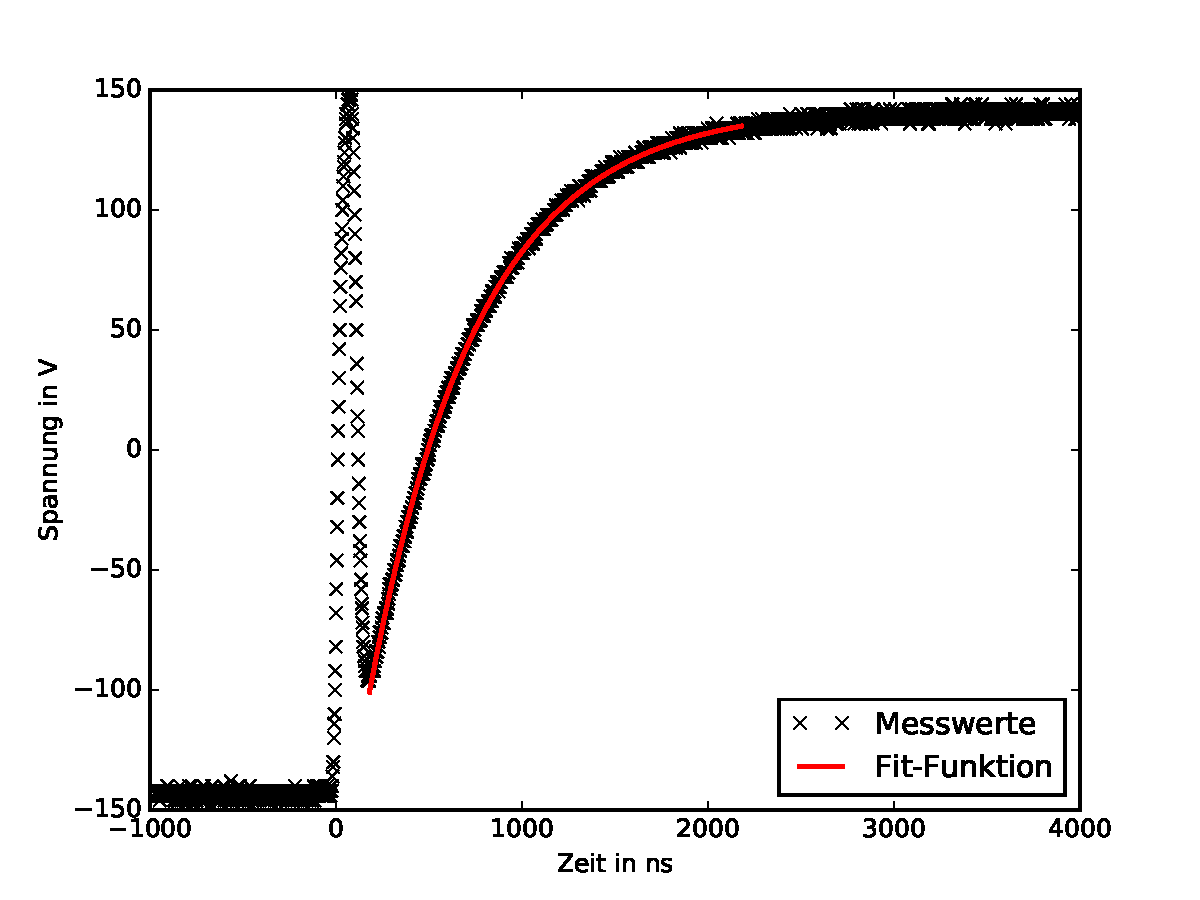
\includegraphics[width=0.7\textwidth]{Box25/Box25.pdf}
	\caption{Spannungsverlauf bei dem Kabel mit Abschlussimpedanz 1}
	\label{fig:box25}
\end{figure}
\clearpage
\subsubsection{Abschlussimpedanz 2}
Bei dieser Abschlussimpedanz handelt es sich um eine Spule und einen Widerstand, die in Reihe geschaltet sind. Die Fit-Funktion ist die selbe wie in Kapitel \ref{sec:impedanz}. Abb. \ref{fig:box23} zeigt die Messwerte ebenso wie die Fit-Funktion. Die Parameter sind:
\begin{align}
	a &= \SI{-12.6127}{\volt}
 \\
	b &= \SI{1.1270}{}
 \\
	c &= \SI{0.0017}{\per\farad\per\ohm}
 \\
	d &= \SI{-9.8317}{\nano\second}
 \\
	e &= \SI{1339.6486}{\volt}
 
\end{align}
Daraus ergibt sich hier für den Widerstand und die Induktivität:
\begin{align}
	R &= \frac{Z_0}{b} - Z_0 = \SI{18.3527}{\ohm}
 \\
	L &= \frac{1}{ c (r + Z_0) \cdot 10^9} = \SI{3.6938}{\micro\henry}
 \quad.
\end{align}

\begin{figure}
	\centering
	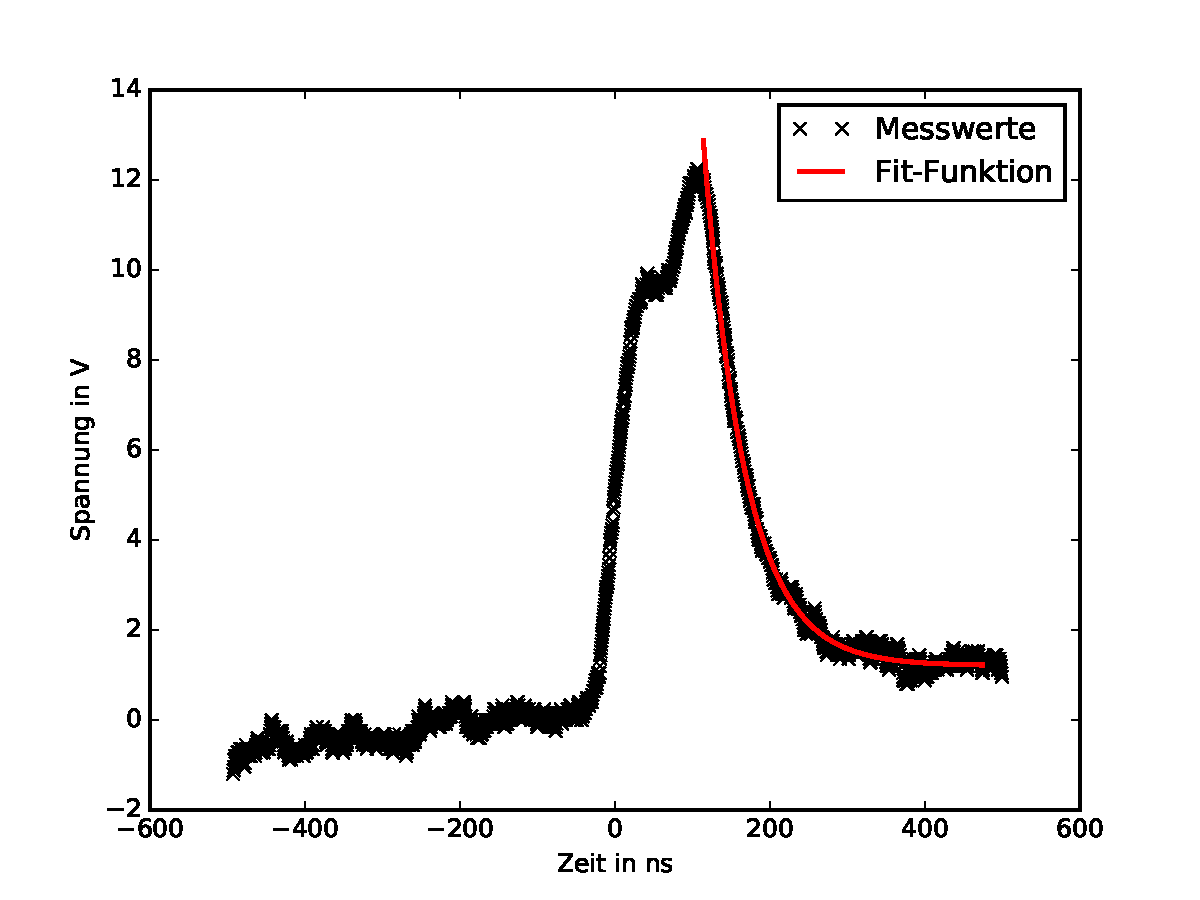
\includegraphics[width=0.7\textwidth]{Box23/Box23.pdf}
	\caption{Spannungsverlauf bei dem Kabel mit Abschlussimpedanz 2}
	\label{fig:box23}
\end{figure}
\clearpage
\subsubsection{Abschlussimpedanz 3}
Bei dieser Abschlussimpedanz handelt es sich, wie bei der Abschlussimpedanz 2, um eine Spule und einen Widerstand, die in Reihe geschaltet sind. Die Rechnungen sind also äquivalent. Abb. \ref{fig:box28} zeigt die Messwerte und die Fit-Funktion. Die Parameter lauten:
\begin{align}
	a &= \SI{-12.6127}{\volt}
 \\
	b &= \SI{1.1270}{}
 \\
	c &= \SI{0.0017}{\per\farad\per\ohm}
 \\
	d &= \SI{-9.8317}{\nano\second}
 \\
	e &= \SI{1339.6486}{\volt}
 
\end{align}
Auch für diese Abschlussimpedanz wird der Widerstand und die Induktivität berechnet:
\begin{align}
	R &= \frac{Z_0}{b} - Z_0 = \SI{18.3527}{\ohm}
 \\
	L &= \frac{1}{ c (r + Z_0) \cdot 10^9} = \SI{3.6938}{\micro\henry}
 \quad.
\end{align}

\begin{figure}
	\centering
	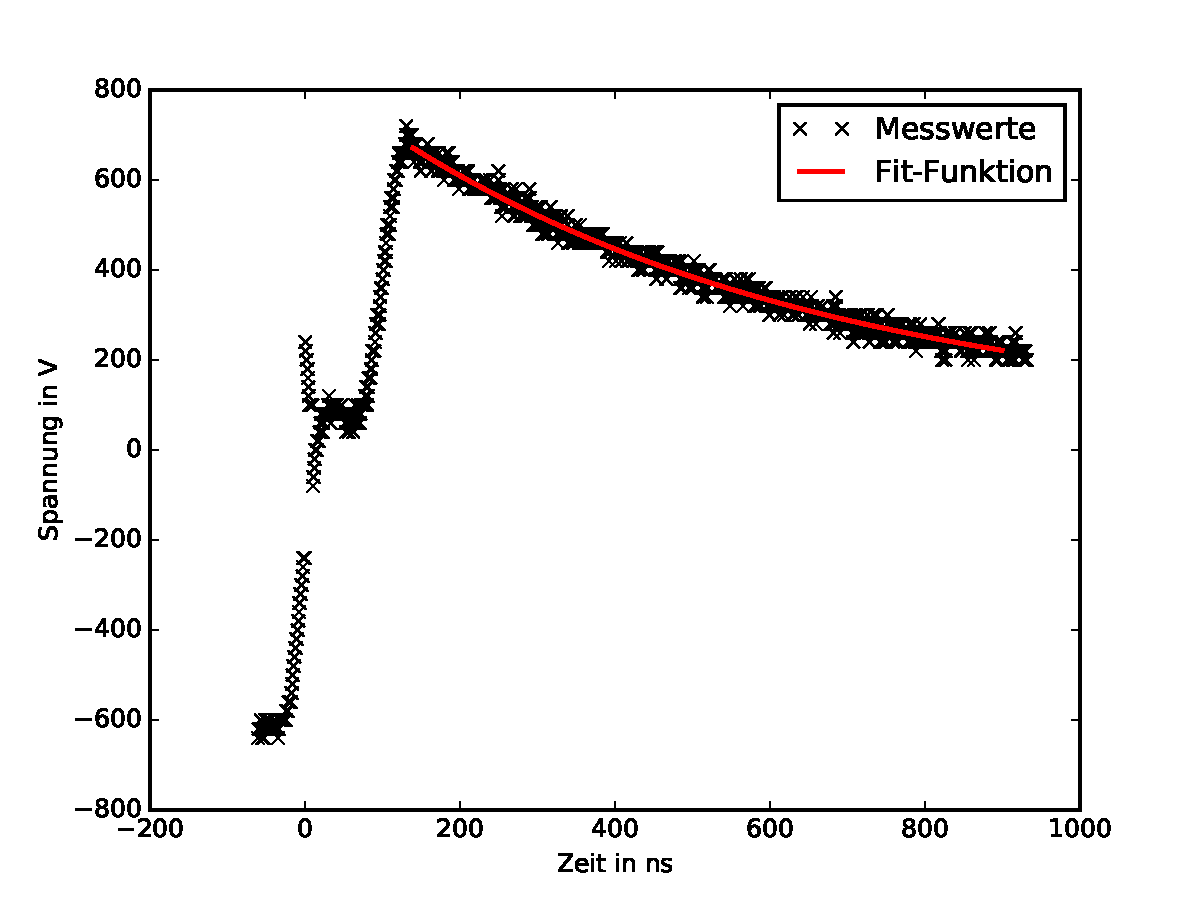
\includegraphics[width=0.7\textwidth]{Box28/Box28.pdf}
	\caption{Spannungsverlauf bei dem Kabel mit Abschlussimpedanz 3}
	\label{fig:box28}
\end{figure}


\clearpage



\clearpage


\section{Diskussion}
Tabelle \ref{tab:Vergleich} zeigt die bestimmten Größen und vergleicht sie mit den Theoriewerten aus den angegebenen Referenzen. Die Bestimmung der Landé-Faktoren und der Kernspins ergibt sehr gute Werte, deren Vertrauensintervalle (mit Ausnahme von $g_{F2}$) den Theoriewert einschließen. Der Wert für das Erdmagnetfeld ist erstaunlich gut, wird bedacht, dass Messungen des Erdmagnetfelds üblicherweise um Größenordnungen abweichen. Das Isotopenverhältnis im Experiment entspricht nicht dem natürlichen Isotopenverhältnis. \\
Die Spin-Bahn-Wechselwirkung muss nicht berücksichtigt werden. Die Untersuchung des quadratischen Zeeman-Effekts zeigt, dass der Effekt für so kleine Magnetfelder, wie sie hier verwendet werden, keine Bedeutung hat.
\begin{table}
	\centering
	\begin{tabular}{lccccc}
		\toprule
		Größe (Referenz) & & Experiment & Theorie & Referenz & Abweichung \\
		\hline
		Landé-Faktor \eqref{eq:LandeExp}& $g_{F1}$ & \SI{0.50+-0.01}{}
 & $\nicefrac{1}{2}$ & \cite{Lande} & $\pm$\SI{0.0}{\%} \\
		& $g_{F2}$ & \SI{0.35+-0.01}{}
 & $\nicefrac{1}{3}$ & \cite{Lande} & +\SI{5.0}{\%} \\
		Erdmagnetfeld \eqref{eq:BErdeExp} & $B_\text{Erde}$ & \SI{30+-2}{\micro\tesla}
 & \SI{49}{\micro\tesla} & \cite{BErde} & \SI{-38.8}{\%} \\
		Kernspin \eqref{eq:KernspinExp} & $I_1$ & \SI{1.51+-0.06}{}
 & $\nicefrac{3}{2}$ & \cite{Ru} & +\SI{0.7}{\%} \\
		& $I_2$ & \SI{2.4+-0.1}{}
 & $\nicefrac{5}{2}$ & \cite{Ru} & \SI{-4.0}{\%} \\
		Isotopenverhältnis \eqref{eq:RatioExp} & $\nicefrac{N_{85}}{N_{87}}$ & \SI{1.5+-0.2}{}
 & 2.6 & \cite{Ru} & \SI{-42.3}{\%} \\
		\bottomrule
	\end{tabular}
\caption{Vergleich der berechneten Größen mit Theoriewerten}
\label{tab:Vergleich}
\end{table}

\clearpage
\listoftodos
\listoffigures
\listoftables
\clearpage
\nocite{\V}
\printbibliography[title = Literaturverzeichnis]

\end{document}
